\documentclass[a4paper, utf8]{article}
\author{Kim Rune Solstad}
\title{Assignment 6, TDT4205}
\usepackage{tikz}
\usepackage[utf8]{inputenc}
\usepackage{graphicx, listings, multirow}
\usetikzlibrary{positioning}
\tikzset{blue node/.style={circle, fill=blue!20,draw,minimum size=1cm, inner sep=0pt}, }
\tikzset{green node/.style={circle, fill=green!20,draw,minimum size=1cm, inner sep=0pt}, }
\tikzset{red node/.style={circle, fill=red!20,draw,minimum size=1cm, inner sep=0pt}, }
\tikzset{yellow node/.style={circle, fill=yellow!20,draw,minimum size=1cm, inner sep=0pt}, }
\begin{document}
\maketitle
\section{Type checking}
To catch the problem in err\_callFunc, we can check return types. Also typecheck for classes has not been implemented.



\section{Symbol tables and blocks}
\subsection{Show the content of the symbol tables at position 1 and 2 assuming a implementation using a stack of symbol tables.}

\subsubsection*{Position 1}
Scope A \\
\begin{tabular}{|l l l|}
	\hline
	\multicolumn{3}{|l|}{\textbf{Function table}} \\
	Name & Type & Attributes	\\
	\hline
	main & void & 			\\
	\hline
	\multicolumn{3}{|l|}{\textbf{Variable table}} \\
	Name & Type &			\\
	\hline
	a & INT &			\\
	b & FLOAT &			\\
	\hline
	\multicolumn{2}{|l}{\textbf{Scope}} & B \\
	\hline
\end{tabular} \\ 
Scope B \\

\begin{tabular}{|l l l|}
	\hline
	\multicolumn{3}{|l|}{\textbf{Function table}} \\
	Name & Type & Attributes	\\
	\hline
	main & void & 			\\
	\hline
	\multicolumn{3}{|l|}{\textbf{Variable table}} \\
	Name & Type &			\\
	\hline
	a & INT &			\\
	b & FLOAT &			\\
	\hline
\end{tabular}

\subsubsection*{Position 2}
Scope A \\
\begin{tabular}{|l l l|}
	\hline
	\multicolumn{3}{|l|}{\textbf{Function table}} \\
	Name & Type & Attributes	\\
	\hline
	main & void & 			\\
	\hline
	\multicolumn{3}{|l|}{\textbf{Variable table}} \\
	Name & Type &			\\
	\hline
	a & INT &			\\
	b & FLOAT &			\\
	\hline
	\multicolumn{2}{|l}{\textbf{Scope}} & C \\
	\hline
\end{tabular} \\
Scope C \\
\begin{tabular}{|l l l|}
	\hline
	\multicolumn{3}{|l|}{\textbf{Variable table}} \\
	Name & Type &			\\
	\hline
	b & INT &			\\
	c & FLOAT &			\\
	\hline
	\multicolumn{2}{|l}{\textbf{Scope}} & D \\
	\hline
\end{tabular} \\
Scope D \\
\begin{tabular}{|l l l|}
	\hline
	\multicolumn{3}{|l|}{\textbf{Variable table}} \\
	Name & Type &			\\
	\hline
	a & BOOL &			\\
	c & INT &			\\
	\hline
\end{tabular}

\subsection*{b)}
\subsubsection*{Position 1}
\begin{tabular}{|l l l l l|}
	\hline
	\multicolumn{5}{|l|}{\textbf{Symbol table}} \\
	Number & Name & Kind & Type & Scope	\\
	\hline
	1 & main & FUNC & VOID & A \\
	2 & a & VAR & INT & A \\
	3 & b & VAR & FLOAT & A \\
	4 & b & VAR & BOOL & B \\ 
	\hline
\end{tabular}

\subsubsection*{Position 2}
\begin{tabular}{|l l l l l|}
	\hline
	\multicolumn{5}{|l|}{\textbf{Symbol table}} \\
	Number & Name & Kind & Type & Scope	\\
	\hline
	1 & main & FUNC & VOID & A \\
	2 & a & VAR & INT & A \\
	3 & b & VAR & FLOAT & A \\
	4 & b & VAR & INT & C \\
	5 & c & VAR & FLOAT & C \\
	6 & a & VAR & BOOL & D \\
	7 & c & VAR & INT & D \\
	\hline
\end{tabular}
\subsection*{c)}
The disadvantage with using an individual table for each scope, is that we might need to search for a name in a number of symbol tables before the symbol is found. When using a single table, we do not need to chain between different tables to locate a name. Using a single table enable us locate a name faster than when using several. 


\section{Data-flow analysis}
\subsection*{a)}
The definition reaches a point if there is a path from the point immediately following the definition to the point, such that the definition is not killed along that path. The definition might be the place at wich the value of the variable was last defined.
\subsection*{b)}
\begin{tabular}{|l|l|c c c c c |}
\hline
Block	&	gen/kill & $OUT[B]^0$ & $IN[B]^1$ & $OUT[B]^1$ & $IN[B]^2$ & $OUT[B]^2$	\\
\hline										%OUT^0		IN^1	OUT^1	IN^2	OUT^2
\hline							
\multirow{2}{*}{B1} 	& $gen\{d_1, d_2, d_3\}$ 				& 000 000 & 000 000 & 111 000 & 000 101 & 111 100  	\\
			& $kill\{d_5, d_6, d_8, d_{10}, d_{11}, d_{12}\}$  	& 000 000 & 000 000 & 000 000 & 111 101 & 101 000 	\\
\hline	
\multirow{2}{*}{B2} 	& $gen\{d_4, d_5\}$	 				& 000 000 & 111 000 & 011 110 & 111 100 & 011 110  	\\
			& $kill\{d_1, d_{10} \}$  				& 000 000 & 000 000 & 000 000 & 101 000 & 101 000 	\\
\hline
\multirow{2}{*}{B3} 	& $gen\{d_6, d_7\}$					& 000 000 & 011 110 & 001 111 & 011 110 & 001 111  	\\
			& $kill\{d_2, d_8 \}$					& 000 000 & 000 000 & 100 000 & 101 000 & 101 000 	\\
\hline
\multirow{2}{*}{B4} 	& $gen\{d_8, d_9\}$					& 000 000 & 011 110 & 001 110 & 011 110 & 001 110  	\\
			& $kill\{d_2, d_6\}$					& 000 000 & 000 000 & 011 000 & 101 000 & 111 000 	\\
\hline
\multirow{2}{*}{B5} 	& $gen\{d_{10}, d_{12}\}$				& 000 000 & 001 111 & 000 101 & 001 111 & 000 101  	\\
			& $kill\{d_1, d_3, d_5, d_{11}\}$			& 000 000 & 111 000 & 111 101 & 111 000 & 111 101 	\\
\hline
\end{tabular}


\subsection{c)}
The compiler may check if any of the definitions for the variable \emph{b} is reachable at point \emph{p}. If there are any, the variable is a constant. 

\section{Register allocation}

\subsection*{a)}
The variable is live at point \emph{p} if its value could be used along some path in the flow graph starting at \emph{p}. Otherwise the variable is dead at that point. 

\subsection*{b)}

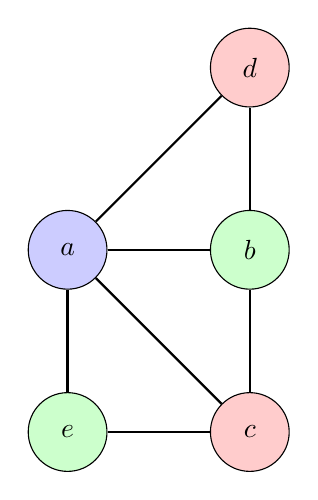
\begin{tikzpicture}
	\node[blue node] (1) {$a$};
	\node[green node] (4) [right = 1.3cm of 1]{$b$};
	\node[red node] (3) [below = 1.3cm of 4]{$c$};
	\node[green node] (2) [left = 1.3cm  of 3]{$e$};
	\node[red node] (5) [above = 1.3cm of 4]{$d$};
	\path[draw,thick]
		(3) edge node {} (1)
		(1) edge node {} (2)
		(2) edge node {} (3)
		(3) edge node {} (4)
		(1) edge node {} (4)
		(4) edge node {} (5)
		(1) edge node {} (5)
		;
\end{tikzpicture}

\subsection*{c)}
After a quick coloring of the interference graph, I have concluded that 3 registers are deeded. 

\end{document}
